\documentclass[12pt]{article}
\usepackage[italian]{babel}
\usepackage{graphicx}
\usepackage{titling}
\usepackage{multicol}
\usepackage{titlesec}
\usepackage{tcolorbox}
\usepackage{hyperref} %To setup table of content links
%\usepackage{changepage}
\usepackage{geometry} %To modify margins


 \geometry{
 a4paper,
 total={170mm,257mm},
 left=20mm,
 top=20mm,
 }

\hypersetup{
    colorlinks,
    citecolor=black,
    filecolor=black,
    linkcolor=black,
    urlcolor=black
}

\newcommand{\sectionbreak}{\clearpage}%To start a section on a new page


\title{Elaborato Assembly}
\author{Stefano Nicolis - Daniele Pasotto}
%=========================================
\begin{document}


\begin{titlepage}
   \begin{center}
       \vspace*{1cm}
 
	\large

      {\huge \textbf{Relazione Progetto E-Shop} }
 
       \vspace{1.5cm}
 
       \textbf{Stefano Nicolis - Alberto Molinari}\\
	\textbf{A.A. 2019-2020}\\
	\vspace{0.35cm}
	\textbf{\today}

\vfill
\begin{figure}[h!]
	\begin{center}
	  
\includegraphics[height=6cm, width=6cm]{media/logounivr}
	\end{center}
\end{figure}
 
	\vfill
 	\textbf{Corso di\\
       Ingegneria del Software\\}
 
       \vspace{3cm}
 
      \begin{multicols}{2}
      \textbf{Università degli Studi di Verona\\
	 Dipartimento di Informatica}
	\end{multicols}
 
   \end{center}
\end{titlepage}


\tableofcontents

\section{Introduzione}
Viene richiesta l'implementazione di un sistema informatico per la gestione del servizio di spesa on-line di un supermercato. Tale applicazione costituisce un modo per mettere in pratica le conoscenze di Ingegneria del Software acquisite nella seconda parte del corso di Programmazione II, tra le quali metodologie di sviluppo, documentazione e test del software.
\\
Questa applicazione prende il nome di \textbf{E-Shop}.


\section{Sviluppo e attività di test}
L'applicazione è stata sviluppata con metodologia incrementale.
\\
Il codice è stato scritto sia in modo individuale che durante sessioni di pair-programming tramite Skype, svoltesi  ogni circa due giorni durante un lasso di tempo di circa tre settimane.
\\
Ogni sessione di pair programming è stata così strutturata:

\begin{itemize}
\item A turno ognuno spiegava all'altro le parti di applicazione sviluppate indipendetemente concordate nella sessione precedente, esponendo i progressi, eventuali idee avute e problemi incontrati
\item Le due parti di codice venivano integrate in un progetto unico, condiviso con l'altro e testato subito su Windows e Ubuntu
\item Le nuove parti di codice da implementare venivano determinate, si iniziava a svilupparle assieme nell'ultima parte della sessione per poi terminare in maniera autonoma entro la sessione successiva
\end{itemize}

La durata media di una sessione era di due ore.


\begin{figure}[h!]
	\begin{center}
 	 	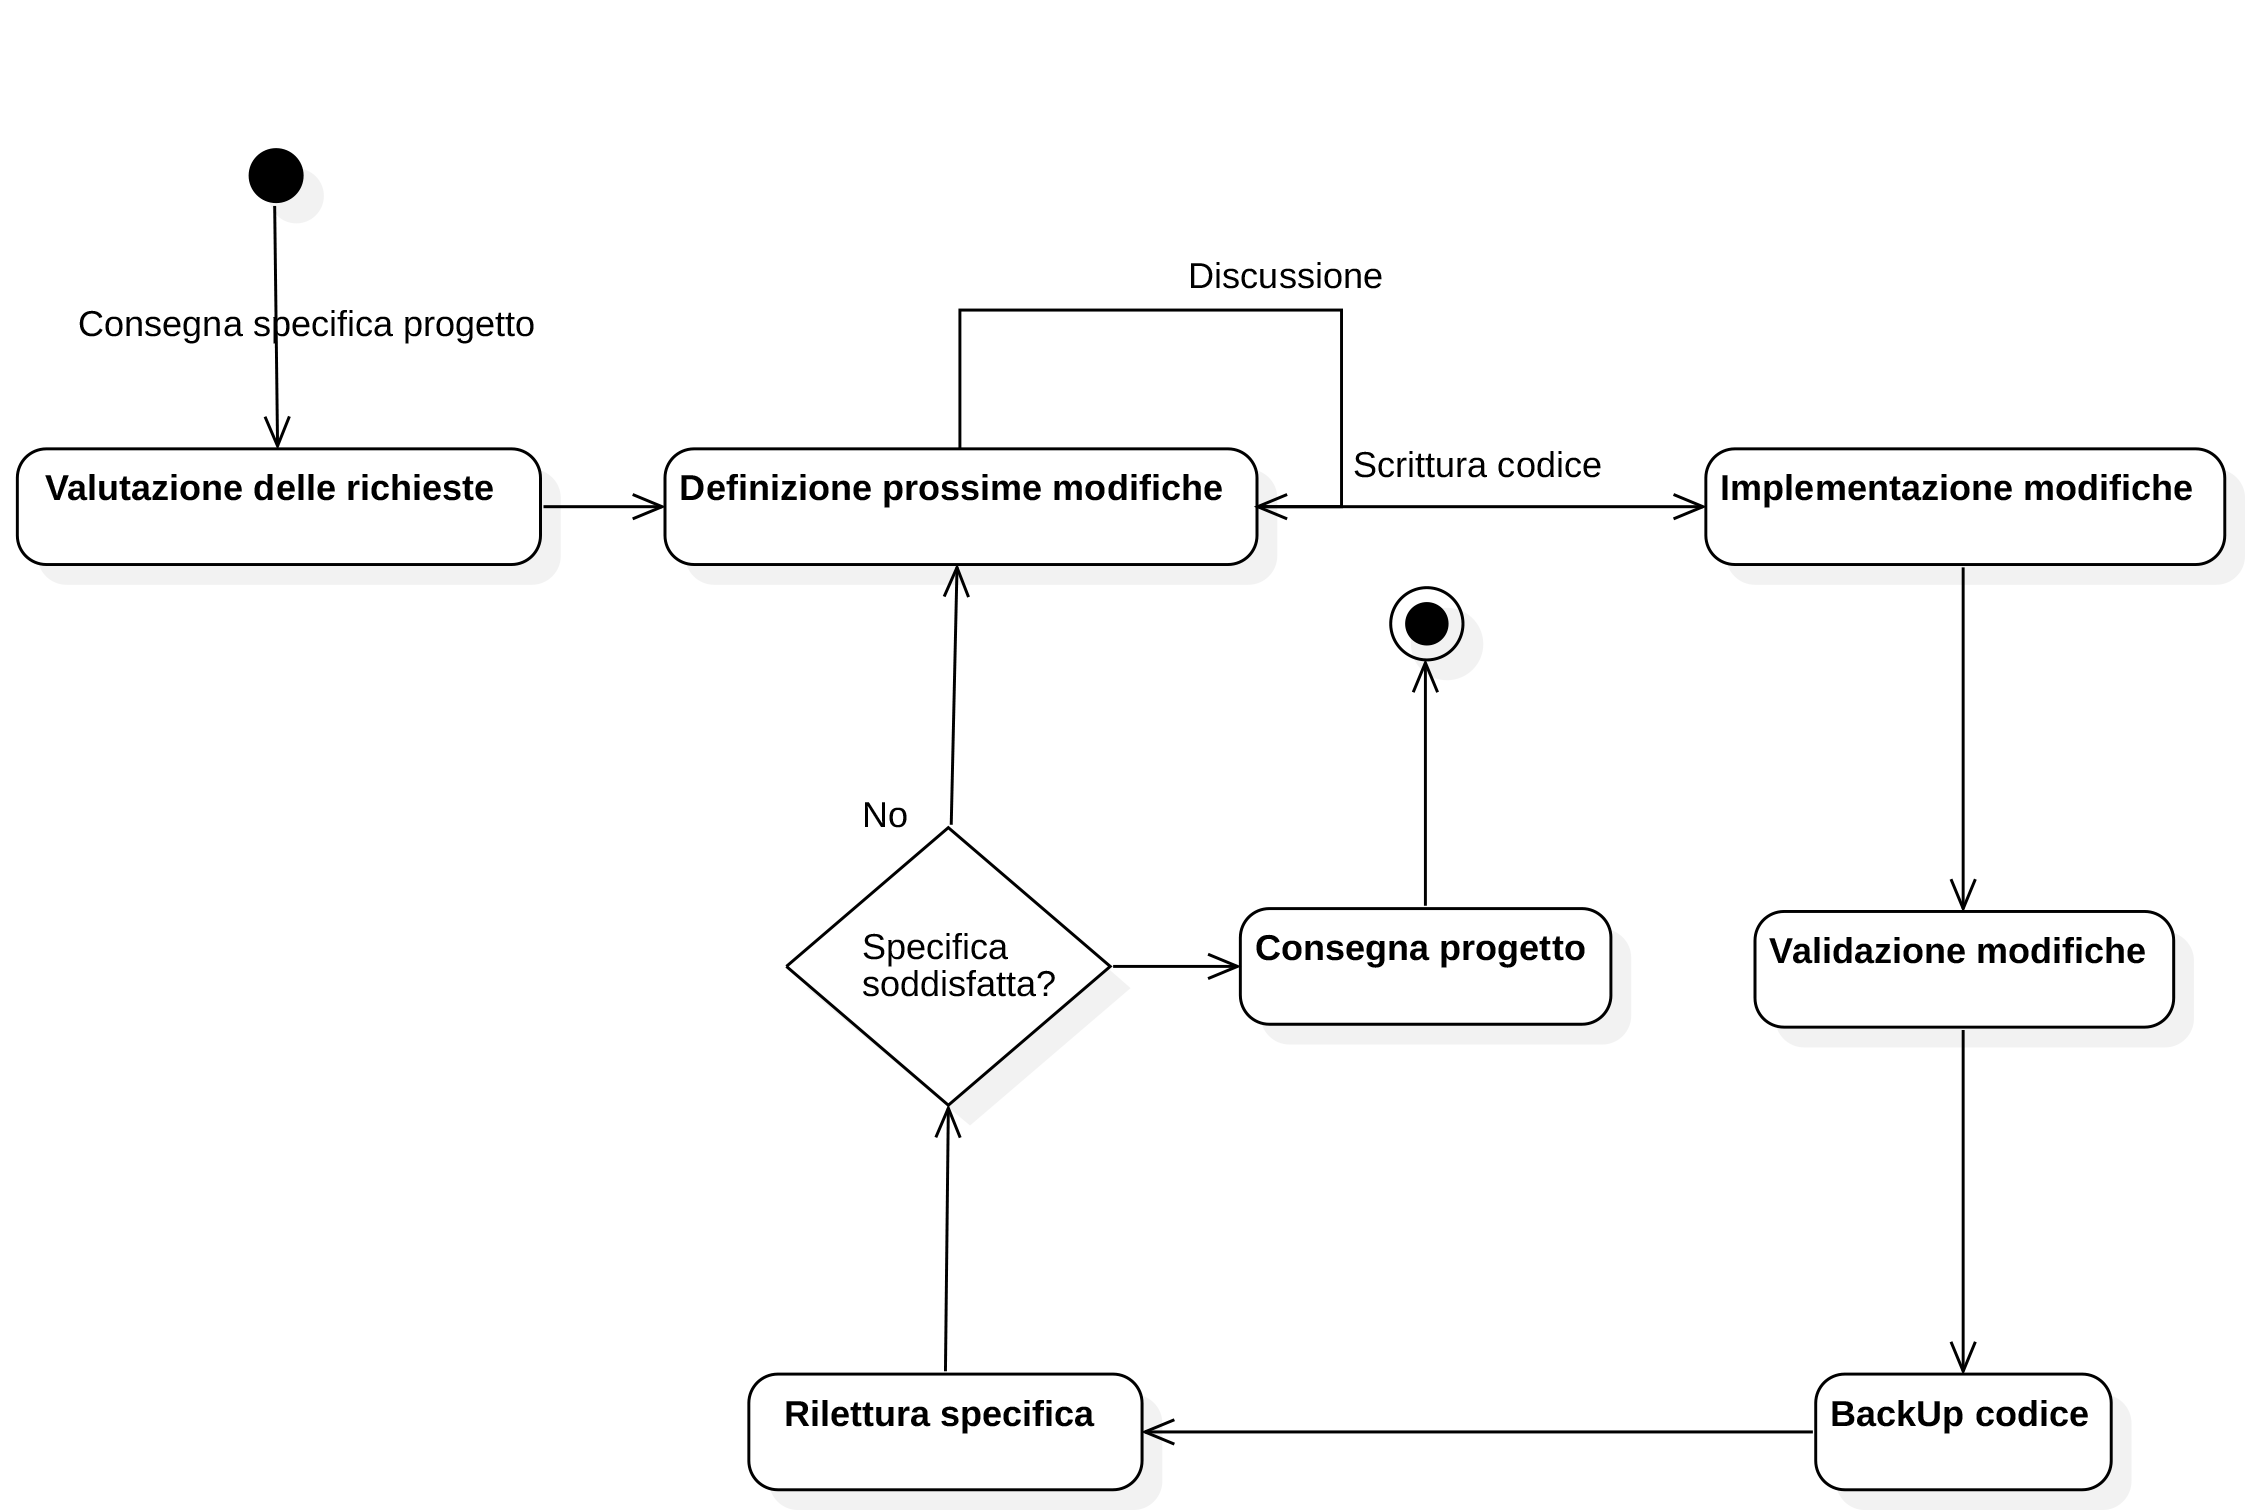
\includegraphics[width=\textwidth,height=\textheight,keepaspectratio]{media/diagrams/activity/developement.png}
  	 	 \caption{Activity Diagram delle attività di sviluppo/test dell'applicazione}
	\end{center}
\end{figure}


\section{Descrizione Software e Scelte Progettuali}
Di seguito vengono elencate le scelte progettuali più significative.

\subsection{Linguaggio di scelta}
Per la realizzazione del progetto è stato scelto il linguaggio \textbf{\emph{Java}} con l'ausilio di \textbf{\emph{JavaFx}} per l'implementazione della parte grafica. La scelta è ricaduta su tali tecnologie perchè, oltre che essere oggetto del corso di studi, tutti i requisiti del progetto erano realizzabili senza problemi con esse, e quindi non abbiamo sentito il bisogno di andare a valutare altre opzioni.

\subsection{Database dei dati}
I vari database dell'applicazione, ovvero la lista degli \textbf{utenti}, dei \textbf{prodotti} e delle \textbf{spese effettuate}, sono realizzati tramite file \textbf{.txt} sui quali vengono scritte le strutture dati utilizzate nel codice, nel nostro caso \textbf{HasMap} contenenti oggetti di tipo \textbf{Product}, \textbf{User} e \textbf{ShoppingCart}. Ciò è permesso dall'implementazione dell'interfaccia \textbf{\emph{Serializable}} da parte degli oggetti presenti nei database.
Abbiamo scelto questo approccio perchè, anche se entrambi avevamo un minimo di esperienza con database relazionali e file xml/json, volevamo fare tutto tramite gli strumenti Java, oltre che sperimentare questo nuovo approccio per la gestione dati che nessuno dei due aveva mai utilizzato prima.

\subsection{Design Pattern e applicazione}
Il design pattern di scelta per eShop è \textbf{Model-View-Control} (MVC): oltre che essere fortemente indicato per l'architettura Vista-Controller di JavaFx, non abbiamo trovato motivo di scegliere altro in quanto esso, oltre ad essere molto facile da usare, ci ha permesso di implementare tutto ciò richiesto dalla specifica con semplicità.

Nel nostro caso, la parte Model è costituita dalle classi del package \emph{models}, ovvero le classi che descrivono gli oggetti che vengono utilizzati nell'applicazione (ad esempio ShoppingCart.java e le enumerazioni Ward.java, PaymentMethod.java), la parte View è costituita dalle viste di JavaFx, ovvero i vari file \textbf{.fxml} del package \emph{views}, e Control sono i rispettivi controllori delle viste contenuti nel package \emph{controllers}.

\subsection{Tipi di utenza}
Gli utenti sono suddivisi in clienti (Customer) e dipendenti (Employee).
\begin{itemize}
\item \textbf{Customer}: può effettuare una spesa all'interno dello shop, controllare il proprio record spese e verificare lo stato degli ordini
\item \textbf{Employee}: può controllare le spese effettuate dai Customer, aggiungere e rimuovere prodotti dallo shop e modificare alcune informazioni come il prezzo e la quantità disponibile dei prodotti già presenti nel database.
\end{itemize}

Entrambe le categorie hanno a disposizione delle credenziali con cui possono effettuare l’autenticazione: i clienti per accedere al sistema usano le credenziali create in fase di registrazione, mentre i dipendenti usano le credenziali fornite dagli amministratori del sistema. Nel caso in cui l’autenticazione vada a buon fine, ogni categoria di utenti viene reindirizzata alla corrispondente interfaccia.

\subsection{Istanze multiple}
L'integrità dei database in presenza di istanze multiple dell'applicazione viene garantina nei seguenti modo:
\begin{itemize}
\item \textbf{Utenti loggati}: all'interno della classe User è presente una flag che viene messa a true quando un utente fa il login e false quando fa il logout, in questo modo non è possibile loggarsi con la stessa utenza in due istanza diverse del programma contemporaneamente.
\item \textbf{Prodotti disponibili}: quando un Customer si logga, viene letto il database dei prodotti da file e caricati i prodotti nella GUI dello shop, a momento di pagamento viene letta una nuova istanza del databse dei prodotti per assicurarsi che i prodtotti scelti dal Customer corrente siano effettivamente ancora disponibili, ovvero verificare che un'altro utente non abbia nel frattempo effettuato una spesa che renda parzialmente o complementamente non soddisfabile la quantità dei prodotti richiesti dall'utente corrente.
\end{itemize}

\subsection{Note utili}
\begin{itemize}
\item Tutti i file utilizzati dall'applicazione, .txt e .png, vengono caricati come risorsa all'interno dell'applicazione e non come oggetti File.
\item Le icone utilizzate nell'applicazione sono state prese da un sito di immagini stock.
\end{itemize}

\section{Viste principali}
Di seguito vengono elencate le principali viste utilizzate.
\subsection{Login.fxml}
Questa vista rappresenta un'interfaccia comue a Customer ed Employee per il login. Un utente non registrato può accedere alla vista Registration.fxml tramite l'apposito bottone per registrare una nuova utenza di tipo Customer. Le utenze di tipo Employee si assume vengano inserite dagli sviluppatori, pertanto non è possibile registrare utenze di tipo Employee da questa schermata. Per questioni di test viene fornita una sola utenza Employee con email e password = (8,8)

\begin{figure}[h!]
	\begin{center}
 	 	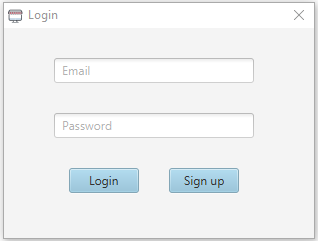
\includegraphics[keepaspectratio]{media/views/login.png}
  	 	 \caption{Vista Login.fxml}
	\end{center}
\end{figure}


\clearpage

\subsection{Registration.fxml}
Tramite questa vista un potenziale utente Customer può registrarsi sulla piattaforma eShop. 
L'utente può scegliere se associare al proprio account una Fidelity Card e un metodo di pagamento preferito.
\\
Si ricorda che \textbf{non} è possibile creare utenze di tipo Employee tramite questa schermata.

\begin{figure}[h!]
	\begin{center}
 	 	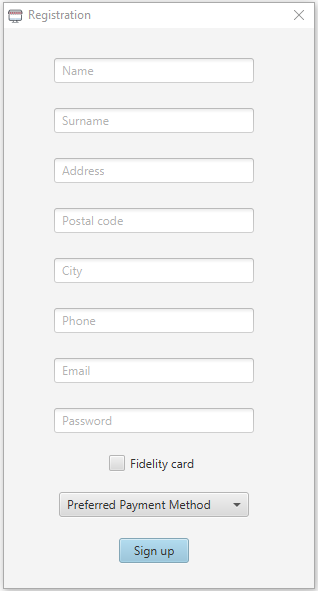
\includegraphics[keepaspectratio]{media/views/registration.png}
  	 	 \caption{Vista Registration.fxml}
	\end{center}
\end{figure}


\clearpage

\subsection{Shop.fxml}
Questa vista rappresenta l'interfaccia grafica per l'utente di tipo Customer.
\\
La schermata è divisa in tre riquadri principali:
\begin{itemize}
\item Sinistra: lista dei prodotti messi nel carrello
\item Centro: vengono visualizzati i prodotti dello shop
\item Destra: informazioni riguardo il prodotto correntemente selezionato
\end{itemize}

\begin{figure}[h!]
	\begin{center}
 	 	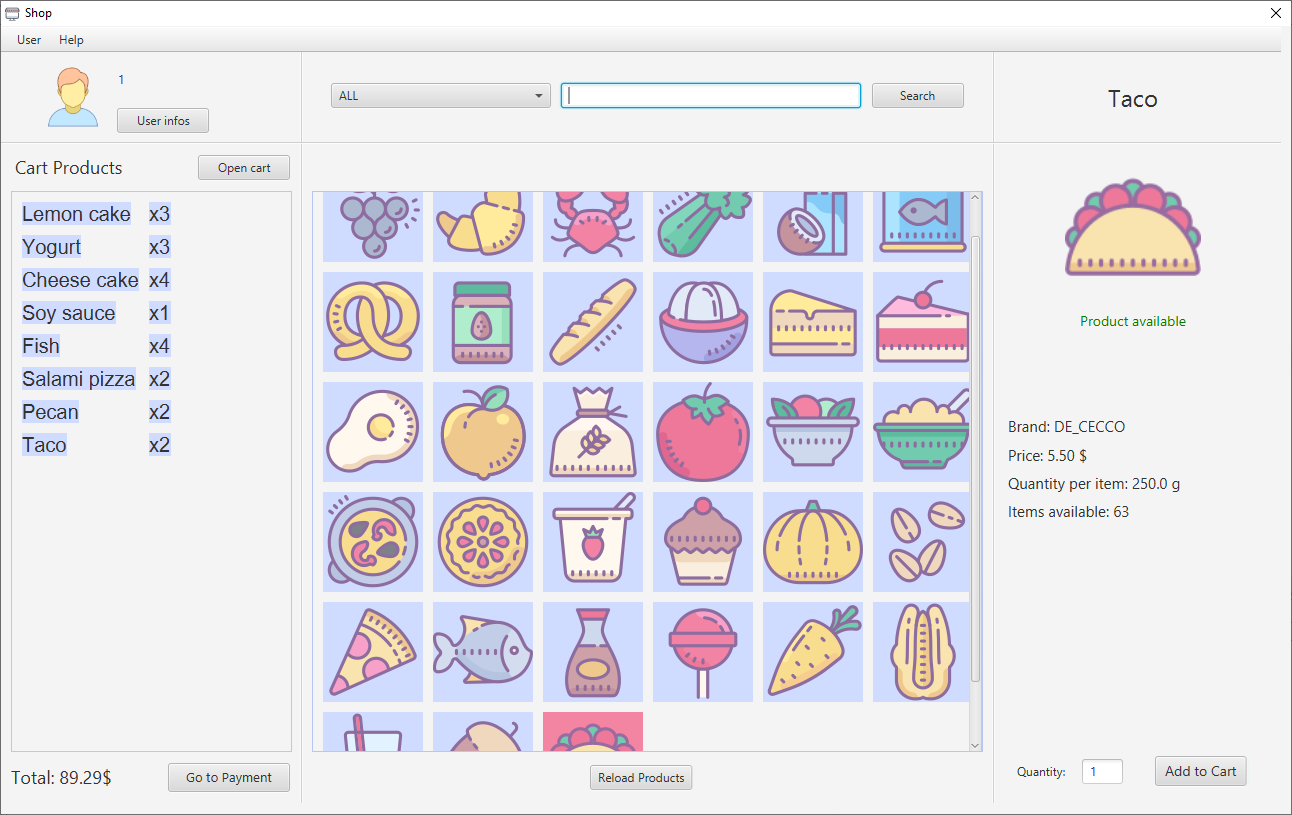
\includegraphics[width=\textwidth, height=\textheight, keepaspectratio]{media/views/shop.png}
  	 	 \caption{Vista Shop.fxml}
	\end{center}
\end{figure}


Per poter aggiungere un prodotto al carrello l'utente deve spostare il cursore sopra il prodotto desiderato, selezionarlo con un click singolo e premere Add to Cart in basso a destra nel pannello del prodotto.
\\
Il tasto \emph{Reload products} serve per aggiornare le quantità visualizzate con le effettive quantità presenti nel database. Se vengono individuati prodotti nel carrello che nel frattempo sono stati comprati, e quindi non più disponibili, essi vengono tolti e un avviso con dettagli viene mostrato all'utente. Lo stesso tipo di controllo viene effettuato al momento del pagamento, vedi sezione Payment.fxml.


\clearpage



\subsection{ShoppingCart.fxml}
Dalla vista \emph{Shop.fxml} il Customer può visualizzare in dettaglio i prodotti che ha messo nel carrello cliccando sul tasto \emph{Open Cart}, questa interfaccia permette di modificare la quantità dei prodotti, rimuoverne uno o più e filtrarli secondo i parametri forniti nella parte alta della vista.

\begin{figure}[h!]
	\begin{center}
 	 	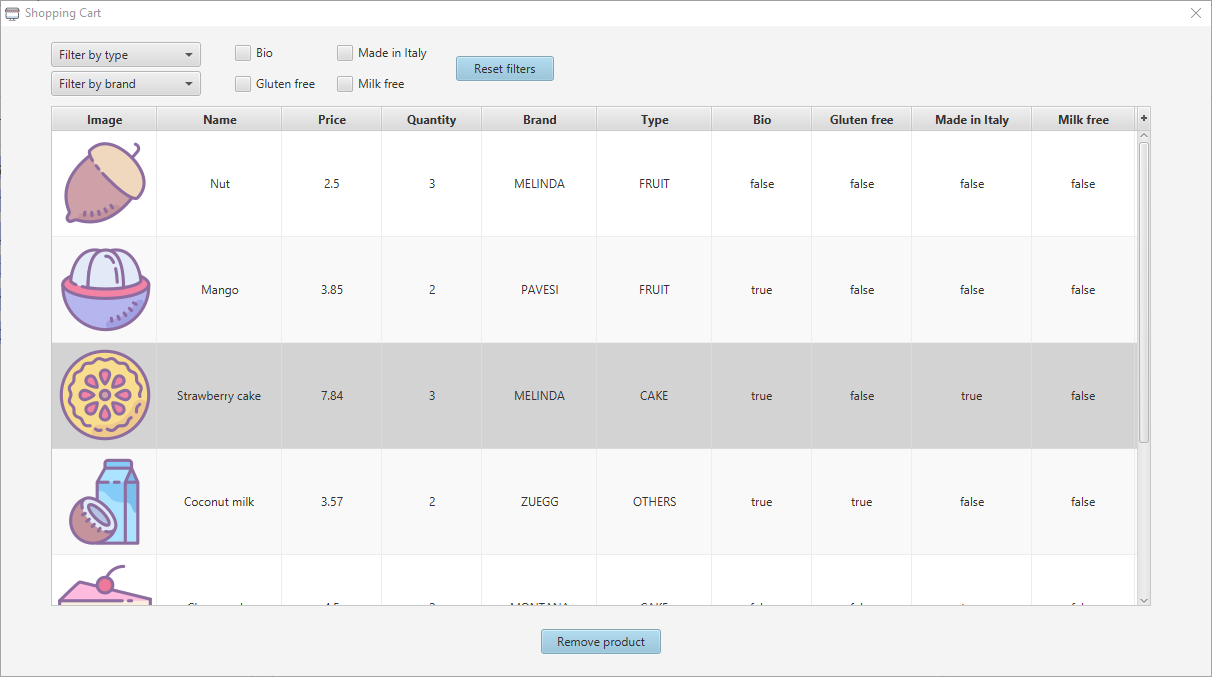
\includegraphics[width=\textwidth,height=\textheight,keepaspectratio]{media/views/shoppingCart.png}
  	 	 \caption{Vista ShoppingCart.fxml}
	\end{center}
\end{figure}


\clearpage

\subsection{Customer.fxml}
Tramite questa vista il Customer può visualizzare la lista di spese effettuate, i prodotti associati a tali spese, e accedere alle viste \emph{FidelityCard.fxml} per visualizzare la propria FidelityCard (se ne esiste una associata al Customer) e \emph{EditProfile.fxml} per modificare le informazioni dell'utente (email, password, etc).
\\
Se in fase di registrazione il customer non ha sottoscritto la carta fedeltà, il sistema disabilita il bottone corrispondente.
\\
È possibile sottoscrivere la carta fedeltà anche in un momento successivo dalla vista \emph{EditProfile.fxml}

\begin{figure}[h!]
	\begin{center}
 	 	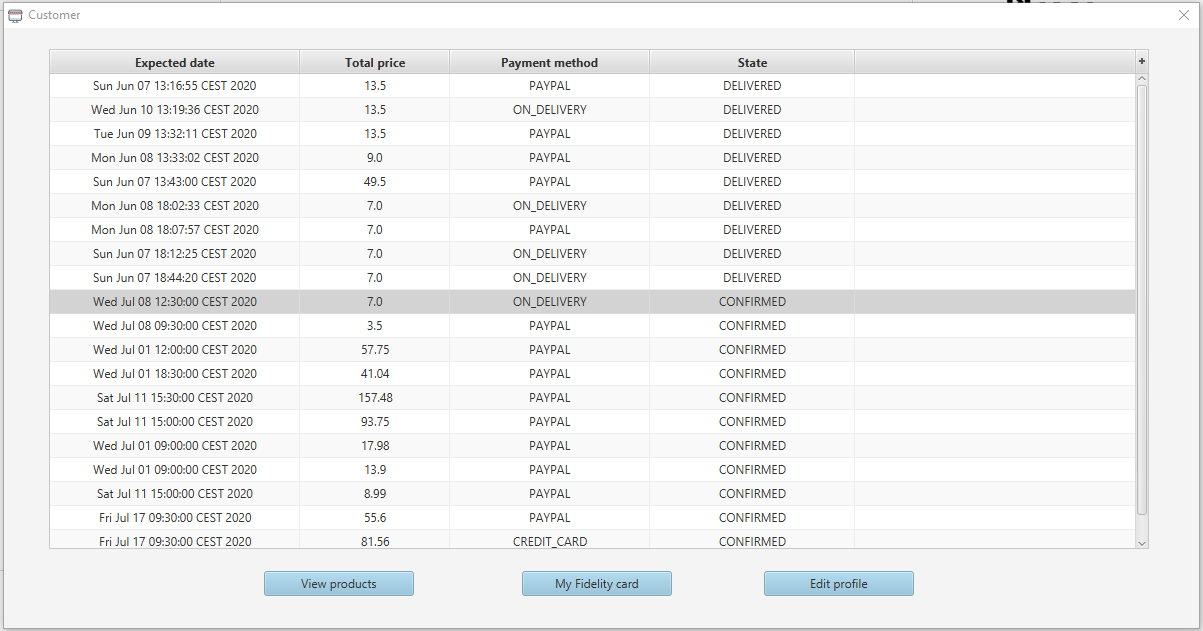
\includegraphics[width=\textwidth,height=\textheight,keepaspectratio]{media/views/customer.png}
  	 	 \caption{Vista Customer.fxml}
	\end{center}
\end{figure}


\clearpage

\subsection{Payment.fxml}
Questa vista permette ai Customer di selezionare una data per la consegna e modalità di pagamento. Per semplicità, le date generate sono random a 1-3 giorni di distanza dalla data di pagamento.

Alla pressione del tasto "Pay" viene inizializzata la sequenza di pagamento:
\begin{itemize}
\item Viene controllata la disponibilità dei prodotti del carrello (nel mentre un'altro utente avrebbe potuto esaurire le scorte che a inizio spesa erano disponibili) e i prodotti non più disponibili vengono tolti dal carrello.
\item Vengono comprati i prodotti (aggiornamento products.txt).
\end{itemize}
Al termine della sequenza di pagamento viene visualizzato un messaggio per informare l'utente che la transazione è andata a buon file, il record della spesa sarà ora disponibile nel file shoppingCarts.txt, visualizzabile dal relativo Customers e i vari Employee.

\begin{figure}[h!]
	\begin{center}
 	 	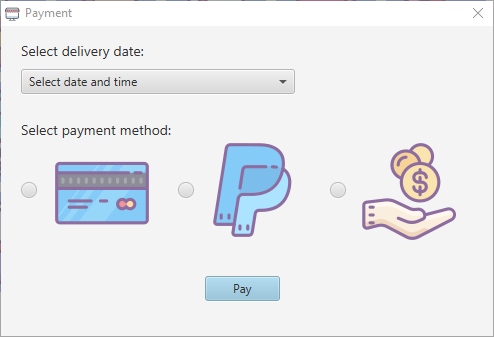
\includegraphics[width=\textwidth,height=\textheight,keepaspectratio]{media/views/payment.png}
  	 	 \caption{Vista Payment.fxml}
	\end{center}
\end{figure}

\clearpage

\subsection{Employee.fxml}
Questa vista fornisce agli Employees la possibilità di:

\begin{itemize}
\item Visualizzare e modificare le informazioni riguardo i prodotti dello shop
\item Aggiungere un nuovo prodotto
\item Visualizzare il database delle spese dei Customer
\end{itemize}

\begin{figure}[h!]
	\begin{center}
 	 	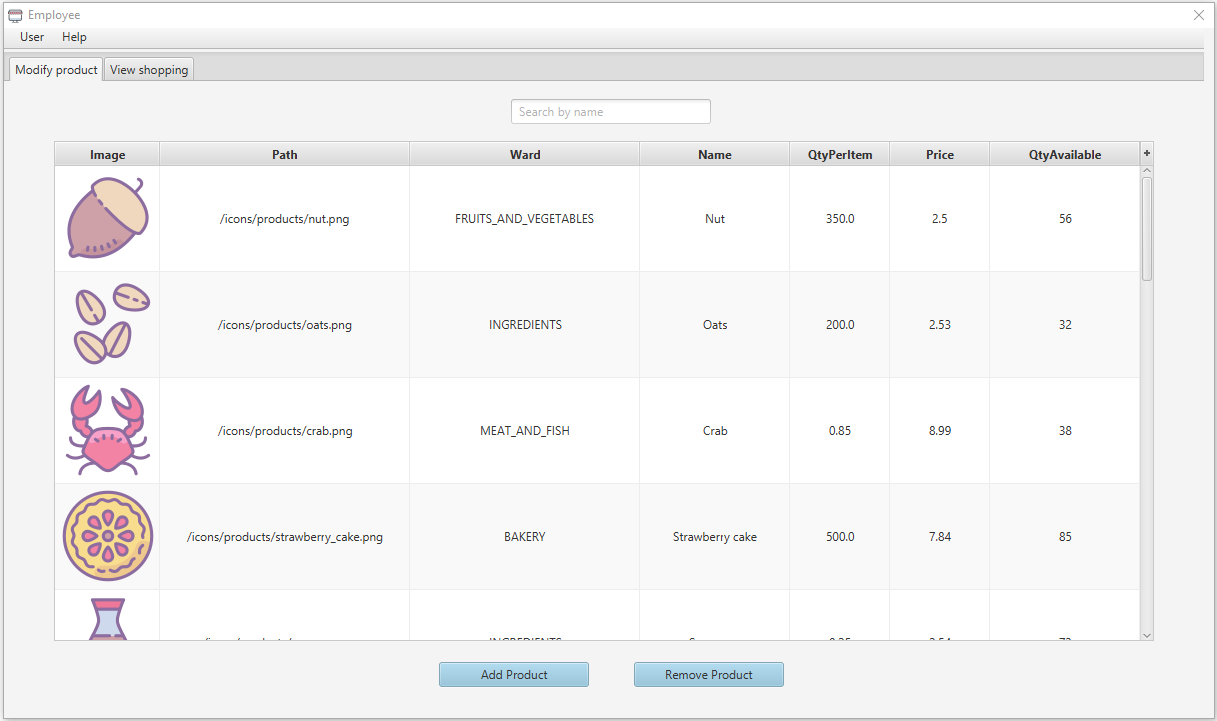
\includegraphics[width=\textwidth,height=\textheight,keepaspectratio]{media/views/employee.png}
  	 	 \caption{Vista Employee.fxml}
	\end{center}
\end{figure}

Si assume che quando l'employee modifichi il database dei prodotti nessun Customer possa fare la spesa, in quanto ciò creerebbe incongruenze nel database.

\section{Casi d'uso}
Di seguito vengono illustrati i casi d'uso del Customer sia in forma di Diagramma che in forma testuale.

\subsection{Casi d'uso relativi al Customer}

\begin{figure}[h!]
	\begin{center}
 	 	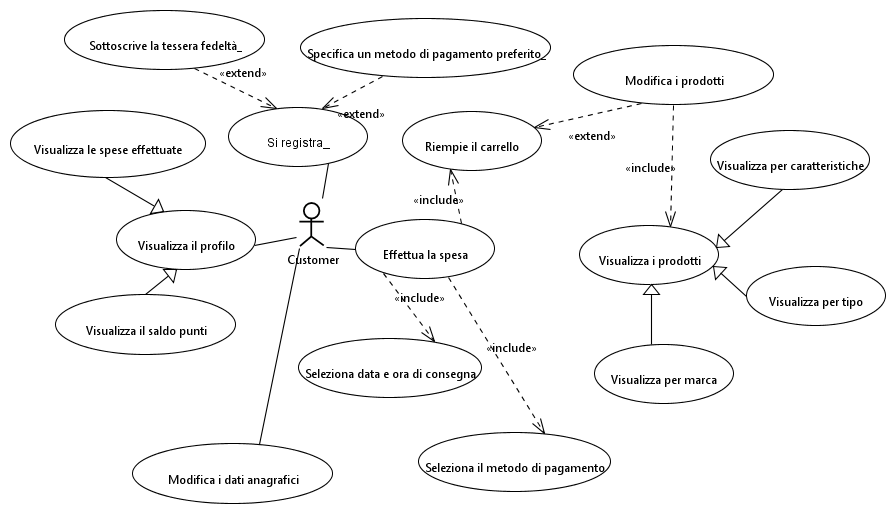
\includegraphics[width=\textwidth,height=\textheight,keepaspectratio]{media/diagrams/use_case/customer.png}
  	 	 \caption{Use case del Customer}
	\end{center}
\end{figure}

\textbf{Visualizza profilo}
\begin{tcolorbox}
\textbf{Precondizioni}: /
	\begin{enumerate}
	\item[1.]	Il customer deve essere autenticato
	\end{enumerate}
\textbf{Sequenza degli eventi}:
	\begin{enumerate}
	\item[1.]	Il caso d’uso inizia quando il customer apre la finestra relativa all’account
	\item[2.]	Se il customer seleziona una spesa effettuata e preme il bottone ‘View products’
 	\item[2.1.]  Il sistema apre una nuova finestra visualizzando i prodotti presenti in quella spesa
 	\item[3.]	Se il customer preme il bottone ‘Fidelity card’
 	\item[3.1.] Il sistema apre una nuova finestra visualizzando i dettagli della carta fedeltà
	\end{enumerate}
\textbf{Postcondizioni}: /
\end{tcolorbox}
\clearpage


\textbf{Registrazione}
\begin{tcolorbox}
	\textbf{Precondizioni}: /
\\
	\textbf{Sequenza degli eventi}:
	\begin{enumerate}
	\item[1.] Il caso d’uso inizia quando il customer apre la finestra di registrazione
	\item[2.] Il customer inserisce le informazioni richieste dal form di registrazione
 	\item[3.] Se il customer sottoscrive la carta fedeltà
 	\item[3.1] Il sistema associa una nuova carta fedeltà al customer
 	\item[4.]  Se il customer seleziona un metodo di pagamento preferito
 	\item[4.1] Il sistema associa il metodo selezionato al customer
 	\item[5.] Il caso d’uso finisce quando il customer preme il bottone ‘Sign up’
	\end{enumerate}
	\textbf{Postcondizioni}: /
\end{tcolorbox}



\textbf{Modifica i prodotti nel carrello}
\begin{tcolorbox}
\textbf{Precondizioni}: Il customer deve aver inserito qualche prodotto nel carrello
\\
\textbf{Sequenza degli eventi}:
	\begin{enumerate}
	\item[1.]  Il caso d’uso inizia quando il customer preme il bottone ‘Open cart’
	\item[2.]  Il customer viene introdotto alla finestra del carrello
 	\item[3.]  Se il customer seleziona uno o più filtri presenti
 	\item[3.1] Il sistema visualizza solo i prodotti che corrispondono ai filtri selezionati
 	\item[4.] Se il customer seleziona un prodotto e digita una nuova quantità
 	\item[4.1] Il sistema aggiorna la quantità del prodotto presente nel carrello
  	\item[5.] Se il customer seleziona un prodotto e preme il bottone ‘Remove Product’
  	\item[5.1] Il sistema rimuove il prodotto selezionato dal carrello
 	\item[6.] Il caso d’uso finisce quando il customer chiude la finestra
	\end{enumerate}
\textbf{Postcondizioni}: Il contenuto del carrello viene aggiornato
\end{tcolorbox}

\clearpage


\textbf{Riempie il carrello}
\begin{tcolorbox}
\textbf{Precondizioni}: Il customer deve essere autenticato
\\
\textbf{Sequenza degli eventi}:
	\begin{enumerate}
	\item[1.] Il caso d’uso inizia quando il customer logga nel sistema
	\item[2.] Il customer viene introdotto all’interfaccia principale
 	\item[3.] Il customer seleziona i prodotti che desidera acquistare e li aggiunge al carrello
	\end{enumerate}
\textbf{Postcondizioni}: Il sistema riempie il carrello con i prodotti selezionati
\end{tcolorbox}



\textbf{Effettuare un'ordine}
\begin{tcolorbox}
\textbf{Precondizioni}: Il customer deve aver aggiunto dei prodotti nel carrello
\\
\textbf{Sequenza degli eventi}:
	\begin{enumerate}
	\item[1.] Il caso d’uso inizia quando il customer preme il bottone ‘Go to Payment’
	\item[2.] Il customer viene introdotto all’interfaccia per il pagamento
 	\item[3.] Il customer seleziona la data e ora di consegna
 	\item[4.] Il customer seleziona una modalità di pagamento
 	\item[5.] Il customer finalizza l’acquisto premendo il bottone 'Pay'
	\end{enumerate}
\textbf{Postcondizioni}: Il sistema registra l'ordine aggiornando i database di prodotti, utenti e spese
\end{tcolorbox}


\clearpage

\subsection{Casi d'uso relativi all'Employee}


\begin{figure}[h!]
	\begin{center}
 	 	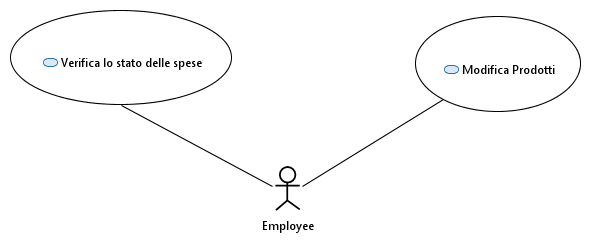
\includegraphics[width=\textwidth,height=\textheight,keepaspectratio]{media/diagrams/use_case/employee.png}
  	 	 \caption{Use case dell'Employee}
	\end{center}
\end{figure}

\textbf{Modifica prodotti}
\begin{tcolorbox}
\textbf{Precondizioni}: L' employee deve essere autenticato
\\
\textbf{Sequenza degli eventi}:
	\begin{itemize}
	\item[1.] Se l' employee preme il bottone "Add Product"
	\item[2.] Se il customer seleziona uno o più filtri presenti
	\item[2.1] Il sistema visualizza solo i prodotti che corrispondono ai filtri selezionati
	\item[3.] Se l' employee digita una nuova quantità
	\item[3.1] Il sistema aggiorna la quantità del prodotto presente nel carrello
	\item[4.] Se l' Employee seleziona un prodotto e preme il bottone "Remove"
	\end{itemize}
\end{tcolorbox}




\section{Sequence diagram per i principali Use Case}

\begin{figure}[h!]
	\begin{center}
 	 	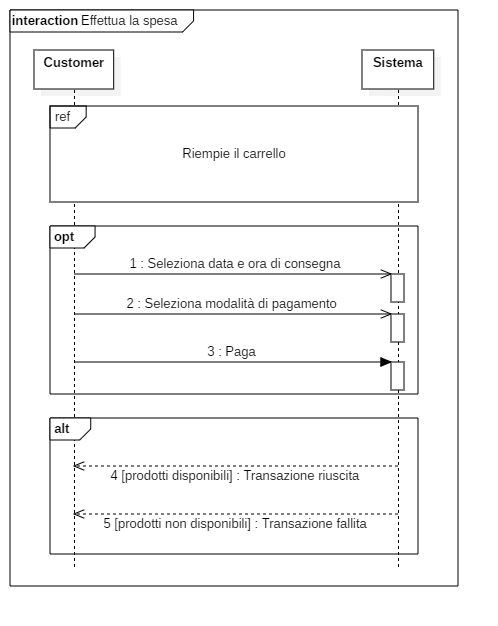
\includegraphics[keepaspectratio]{media/diagrams/sequence/effettua_spesa.png}
  	 	 \caption{Sequence Diagram delle attività di spesa del Customer}
	\end{center}
\end{figure}


\begin{figure}[h!]
	\begin{center}
 	 	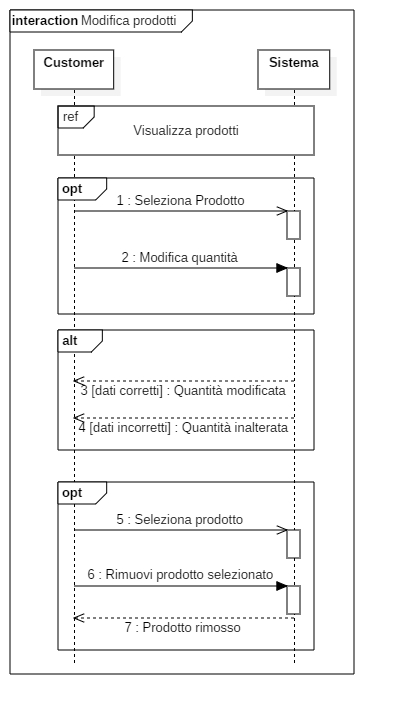
\includegraphics[keepaspectratio]{media/diagrams/sequence/modifica_prodotti.png}
  	 	 \caption{Sequence Diagram della modifica dei prodotti del carello del Customer}
	\end{center}
\end{figure}


\begin{figure}[h!]
	\begin{center}
 	 	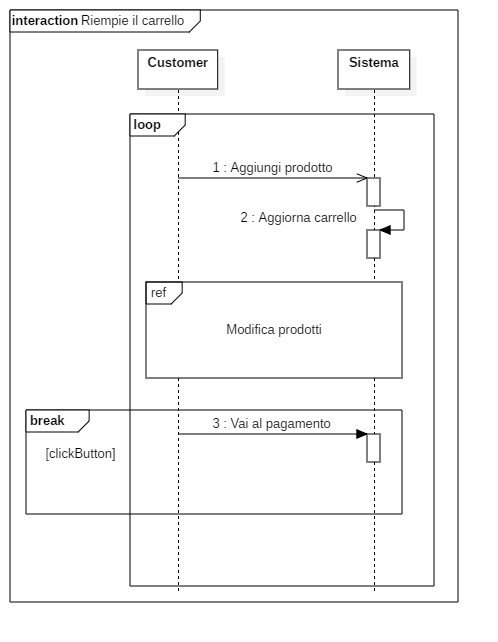
\includegraphics[keepaspectratio]{media/diagrams/sequence/riempi_carrello.png}
	\end{center}
\end{figure}

\begin{figure}[h!]
	\begin{center}
 	 	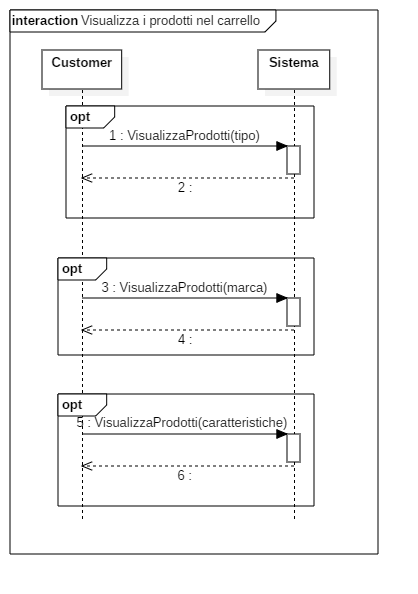
\includegraphics[keepaspectratio]{media/diagrams/sequence/visualizza_prodotti_carrello.png}
	\end{center}
\end{figure}


\section{Application Diagrams}
\subsection{Class Diagram}
Di seguito vengono riportati i Class Diagram di maggior rilevanza
\begin{figure}[h!]
	\begin{center}
 	 	\makebox[\textwidth]{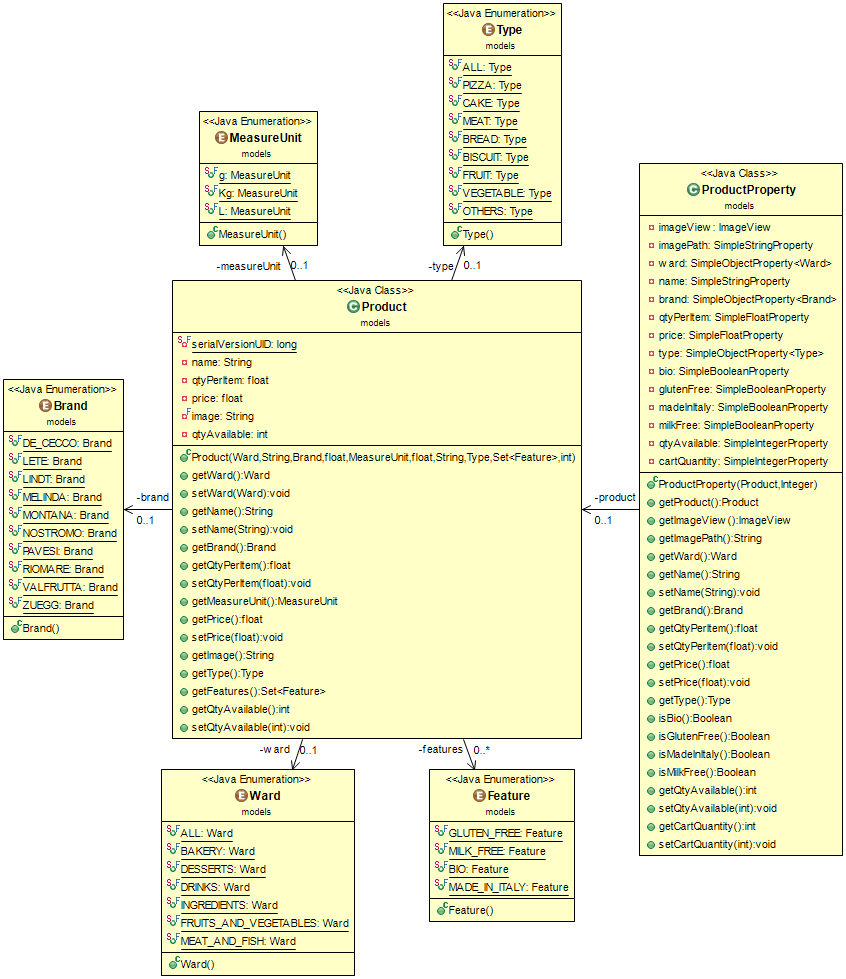
\includegraphics[height=19cm, width=19cm]{media/diagrams/class/product.png}}
  	 	 \caption{Class diagram della logica dei prodotti}
	\end{center}
\end{figure}

\begin{figure}[h!]
	\begin{center}
 	 	\makebox[\textwidth]{
\includegraphics[height=19cm, width=19cm]{media/diagrams/class/user.png}}
  	 	 \caption{Class diagram della logica delle utenze}
	\end{center}
\end{figure}

\end{document}